\documentclass[12pt, a4paper]{article}
\usepackage{amscd, amssymb,amsmath}
\usepackage{booktabs}
\usepackage{graphicx}
\usepackage{xstring}
\usepackage{tikz}
\usetikzlibrary{calc}
\graphicspath{{./img/}}
\emergencystretch=50pt
\allowdisplaybreaks[2]

\addtolength{\topmargin}{-5\baselineskip}
\addtolength{\textheight}{9\baselineskip}
\addtolength{\textwidth}{3cm}
\addtolength{\oddsidemargin}{-15mm}
\addtolength{\evensidemargin}{-15mm}
\addtolength{\parskip}{3pt plus 1pt}

\renewcommand{\theenumi}{\alph{enumi}}

\newcommand{\NodeAA}{\textbf{Node $(1,1)$}}%
\newcommand{\NodeAB}{\textbf{Node $(1,2)$}}%
\newcommand{\NodeAC}{\textbf{Node $(1,3)$}}%
\newcommand{\NodeAD}{\textbf{Node $(1,4)$}}%
\newcommand{\NodeAE}{\textbf{Node $(1,5)$}}%

\newcommand{\NodeBA}{\textbf{Node $(2,1)$}}%
\newcommand{\NodeBB}{\textbf{Node $(2,2)$}}%
\newcommand{\NodeBC}{\textbf{Node $(2,3)$}}%
\newcommand{\NodeBD}{\textbf{Node $(2,4)$}}%
\newcommand{\NodeBE}{\textbf{Node $(2,5)$}}%

\newcommand{\NodeCA}{\textbf{Node $(3,1)$}}%
\newcommand{\NodeCB}{\textbf{Node $(3,2)$}}%
\newcommand{\NodeCC}{\textbf{Node $(3,3)$}}%
\newcommand{\NodeCD}{\textbf{Node $(3,4)$}}%
\newcommand{\NodeCE}{\textbf{Node $(3,5)$}}%

\newcommand{\NodeDA}{\textbf{Node $(4,1)$}}%
\newcommand{\NodeDB}{\textbf{Node $(5,2)$}}%
\newcommand{\NodeDC}{\textbf{Node $(5,3)$}}%
\newcommand{\NodeDD}{\textbf{Node $(5,4)$}}%
\newcommand{\NodeDE}{\textbf{Node $(5,5)$}}%

\newcommand{\NodeEA}{\textbf{Node $(5,1)$}}%
\newcommand{\NodeEB}{\textbf{Node $(5,2)$}}%
\newcommand{\NodeEC}{\textbf{Node $(5,3)$}}%
\newcommand{\NodeED}{\textbf{Node $(5,4)$}}%
\newcommand{\NodeEE}{\textbf{Node $(5,5)$}}%

\newcommand{\Size}{2.5cm}
\def\NumOfColumns{5}%
\def\Sequence{1/A, 2/B, 3/C, 4/D, 5/E}

\tikzset{Square/.style={
    inner sep=0pt,
    text width=\Size +1, 
    minimum size=\Size,
    draw=black,
    fill=yellow!20,
    align=center
    }
}

\begin{document}
\pagestyle{empty}

\begin{center}

   \medskip
   {\large\bf KANANGA BINGO}


   \bigskip
   \medskip
   {
\includegraphics[scale=0.2]{kanangaLogo}}





   \bigskip
   \medskip

   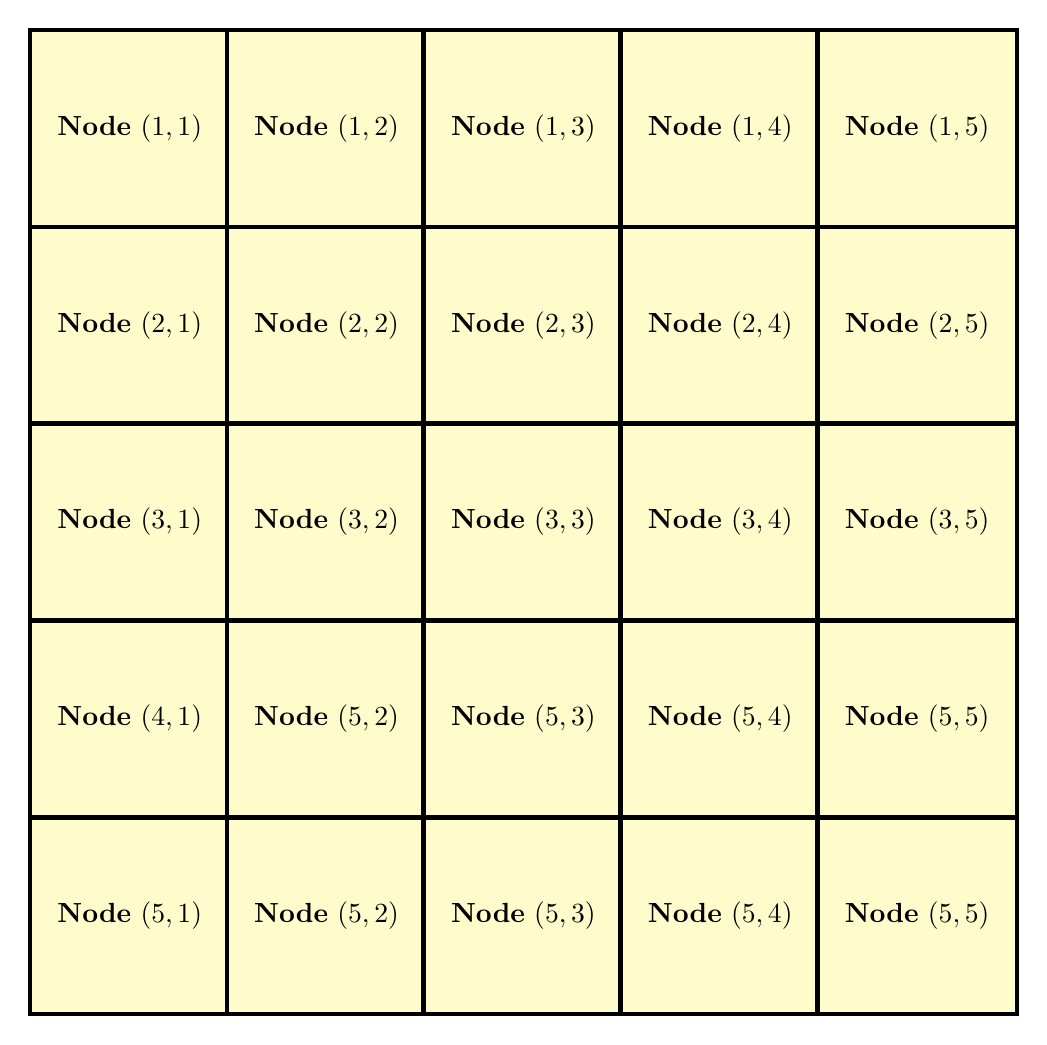
\begin{tikzpicture}[draw=black, ultra thick, x=\Size,y=\Size]
      \foreach \col/\colLetter in \Sequence {%
         \foreach \row/\rowLetter in \Sequence{%
            \pgfmathtruncatemacro{\value}{\col+\NumOfColumns*(\row-1)}
            \def\NodeText{\expandafter\csname Node\rowLetter\colLetter\endcsname}
            \node [Square] at ($(\col,-\row)-(0.5,0.5)$) {\NodeText};
         }
      }
   \end{tikzpicture}
\end{center}
\end{document}
